\documentclass[a4paper,12pt]{article}
\usepackage[spanish]{babel}
\spanishdecimal{.}
\selectlanguage{spanish}
\usepackage[spanish,onelanguage,ruled]{algorithm2e}
\usepackage[utf8]{inputenc}
\usepackage{graphicx}
\usepackage{caption}
\usepackage{subcaption}
\usepackage[top=2cm, bottom=2cm, left=2cm, right=2cm]{geometry}
\usepackage{hyperref}
\usepackage{verbatim}
\usepackage{amssymb}
\usepackage{mathtools}
\usepackage{listings}
\usepackage{color}
\definecolor{backcolour}{rgb}{0.95,0.95,0.92}
\newcommand\ddfrac[2]{\frac{\displaystyle #1}{\displaystyle #2}}
\lstset{backgroundcolor=\color{backcolour}, basicstyle=\footnotesize}
\lstset{xleftmargin=1cm, xrightmargin=1cm, breaklines=true}

\title{Práctica 7 \\ Conexión de actuadores a la tarjeta Arduino Uno}
\author{Laboratorio de Bio-Robótica}
\date{Construcción de Robots Móviles}
\begin{document}
\renewcommand{\tablename}{Tabla}
\maketitle
\section*{Objetivos}
\begin{itemize}
\item Utilizar el circuito DRV8833 como etapa de potencia para los dos motores de corriente directa del robot. 
\item Controlar los dos motores mediante las señales PWM de la tarjeta Arduino Uno.
\item Implementar un nodo de ROS en la tarjeta Arduino Uno que se suscriba a los valores de velocidad deseados para los dos motores. 
\item Utilizar una interfaz gráfica de usuario (GUI) para operar ambos motores. 
\end{itemize}

\section{Introducción}
En un robot autónomo, uno de los sistemas más importantes es el control de bajo nivel de los actuadores, de los cuales, el más común, es el motor de corriente directa. Para controlarlo se requiere de un subsistema que ``traduzca'' las señales enviadas por el sistema de procesamiento a señales de potencia para el control de los motores. Este subsistema se conoce como etapa de potencia. 

La etapa de potencia más utilizada para el control de motores de DC es el circuito puente H, que permite aplicar un voltaje a una carga en ambos sentidos. La figura \ref{fig:PuenteH} muestra la estructura general de este circuito. Se puede observar que si los interruptores S1 y S2 están cerrados y S3 y S4, abiertos, entonces el motor girará en sentido horario. Por el contrario, si se abren s1 y S2, y se cierran S3 y S4, la polaridad sobre el motor se invertirá y éste girará en sentido antihorario. 

Generalmente se utilizan dos señales lógicas para operar los cuatro interruptores. En la figura \ref{fig:PuenteH}, la señal M1 abre o cierra simultáneamente los interruptores S1 y S2 y la señal M2, los interruptores S3 y S4. Al ser señales lógicas, M1 y M2 pueden generarse en la unidad de procesamiento y éstas servirán para mover el motor en ambos sentidos. En la tabla \ref{tab:PuenteH} se resumen los efectos que tienen sobre el motor las diferentes combinaciones de las señales lógicas M1 y M2. 

\begin{figure}
  \centering
  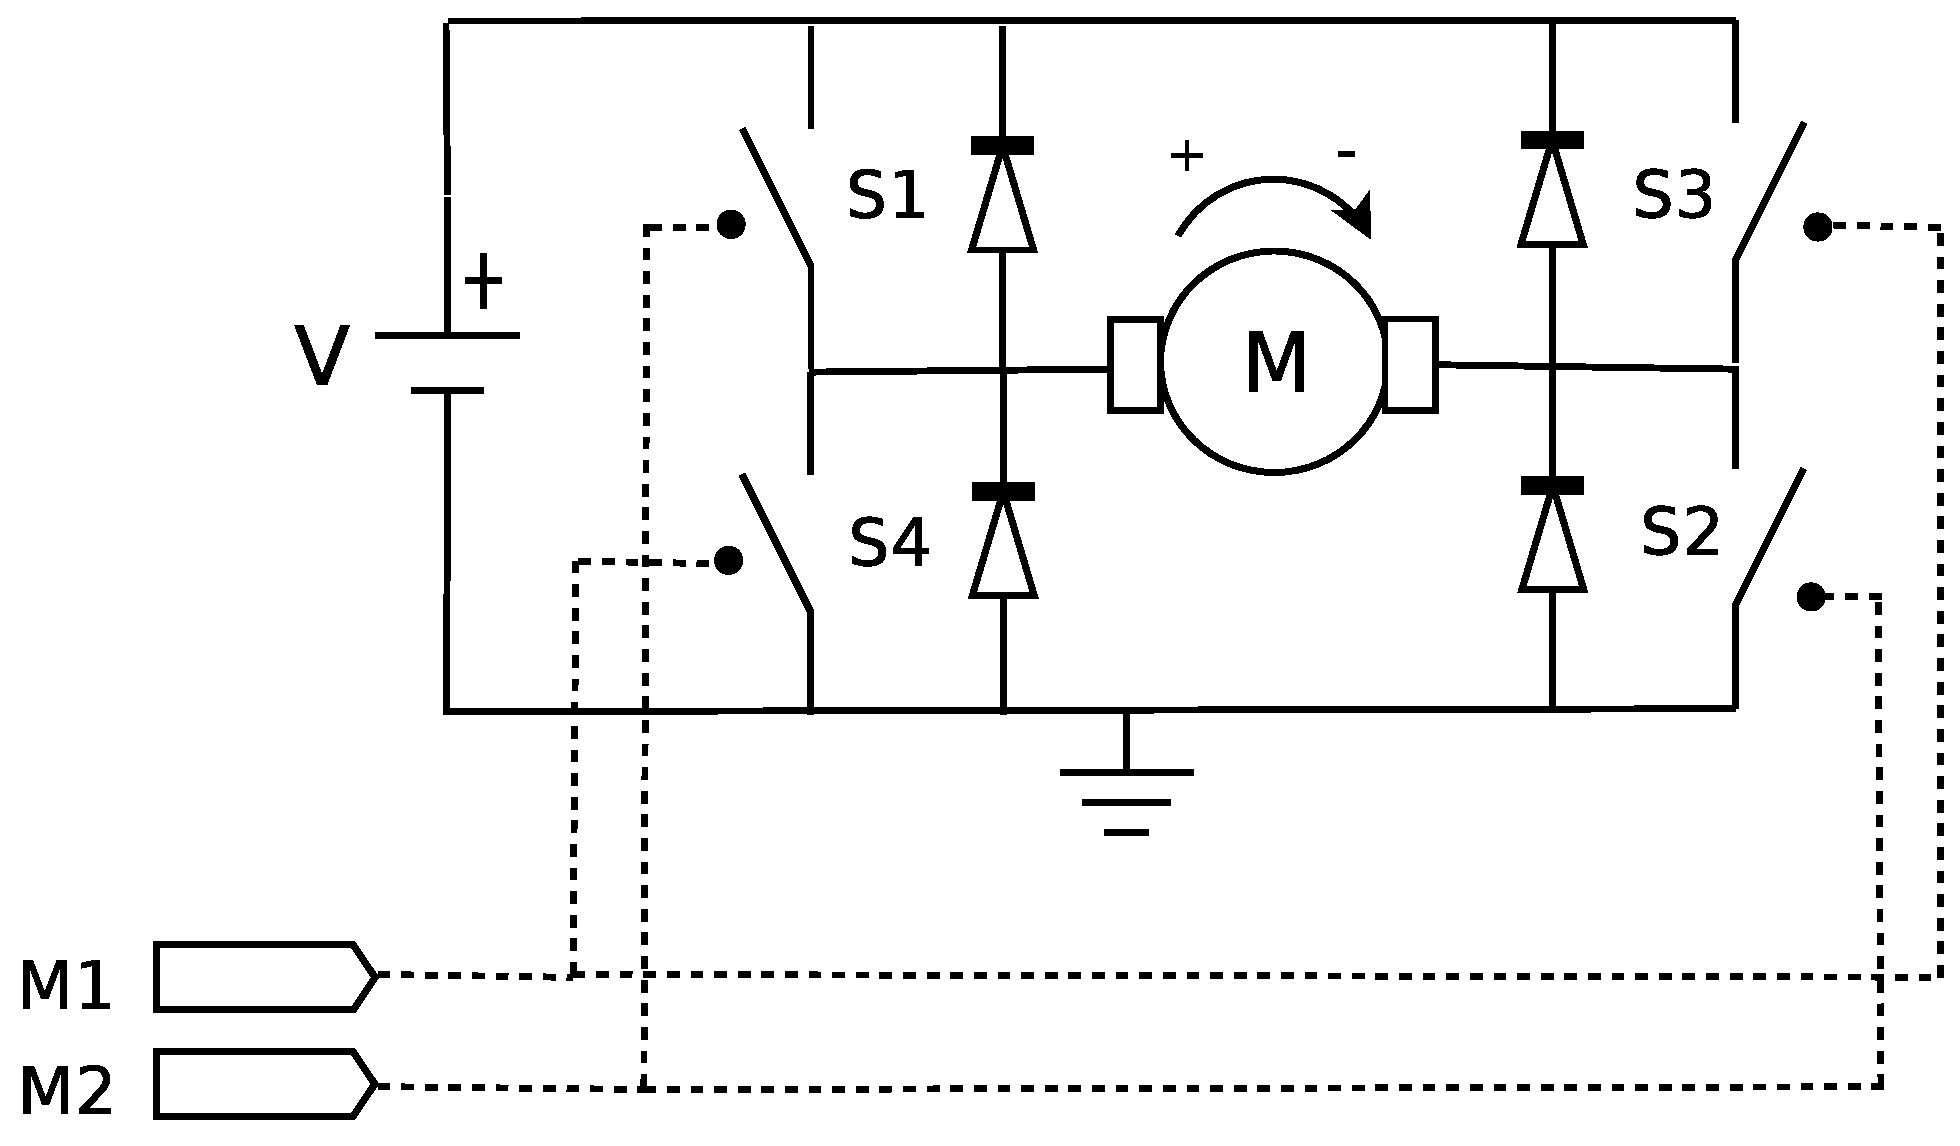
\includegraphics[width=0.5\textwidth]{Figures/PuenteH.eps}
  \caption{El circuito Puente H}
  \label{fig:PuenteH}
\end{figure}

\begin{table}
  \centering
  \begin{tabular}{|rrl|}
    \hline
    M1 & M2 & Efecto sobre el motor\\
    \hline
    0 & 0 & Giro libre\\
    0 & 1 & Movimiento en sentido horario\\
    1 & 0 & Movimiento en sentido antihorario\\
    1 & 1 & Corto circuito\\
    \hline
  \end{tabular}
  \caption{Tabla de verdad para el puente H}
  \label{tab:PuenteH}
\end{table}

Ahora, en un robot móvil, no basta con poder mover el motor en ambos sentidos, sino que es necesario poder controlar su velocidad. Sabemos que en un motor de DC, el par generado es proporcional a la corriente que circula por éste, y la velocidad angular, proporcional al voltaje en sus terminales. Dado que no se puede modificar el voltaje de la bateria arbitrariamente, es necesario utilizar la técnica de modulación por ancho de pulso (PWM por sus siglas en inglés). 



\end{document}

%%% Local Variables:
%%% mode: latex
%%% TeX-master: t
%%% End:
